\section{Corretor numérico}\label{secao:corretor_numerico}

Uma alternativa (ou complemento) ao uso de integradores simpléticos é utilizar integradores tradicionais e aplicar algum tipo de correção a cada passo, de modo a garantir que a solução aproximada conserve as integrais primeiras. O método apresentado nesta seção tem esse propósito, e, embora aqui tenha sido desenvolvido intuitivamente, este foi proposto inicialmente por \cite{Nacozy1972} e posteriormente analisado por \cite{Shampine1986}.

Sejam $\vet z = (\vet q, \vet p)$ um vetor no espaço de fases para um problema de $N$ partículas (não necessariamente o PNCG) e $\vet z_0 = (\vet q_0, \vet p_0)$ o valor inicial de um Problema de Cauchy conservativo
\begin{equation*}
    \dvet z (t) = F(t,\vet z(t)), \quad \vet z(t_0) = \vet z_0,
\end{equation*}
com $F$ suave. Seja também $\vet \Psi (\vet z) = (\psi_1(\vet z), ..., \psi_k(\vet z))$ um conjunto de $k$ integrais primeiras para o problema, sendo $\vet \Psi_0 = \vet \Psi(\vet z_0)$.

Tome um instante $t \in I$, sendo $I$ o intervalo maximal do problema, e considere a solução exata $\vet z^* = \vet z(t)$ e a solução aproximada $\tilde{\vet z}$, obtida através de um integrador numérico qualquer. Espera-se de uma boa simulação conservativa que $\vet z$ seja solução de
\begin{equation}\label{eq:problema_otimizacao_corretor}
    \begin{aligned}
        \min \quad & \norma{\tilde{\vet z} - \vet z^*} \\
        \text{s. a} \quad & \psi_i (\vet z^*) = \psi_i (\vet z_0) \\
        &  i = 1, ..., k.
    \end{aligned}
\end{equation}
Como o que se tem é $\tilde{\vet z}$, podemos analisar em função de $\vet z^*$.

\begin{figure}
    \centering
    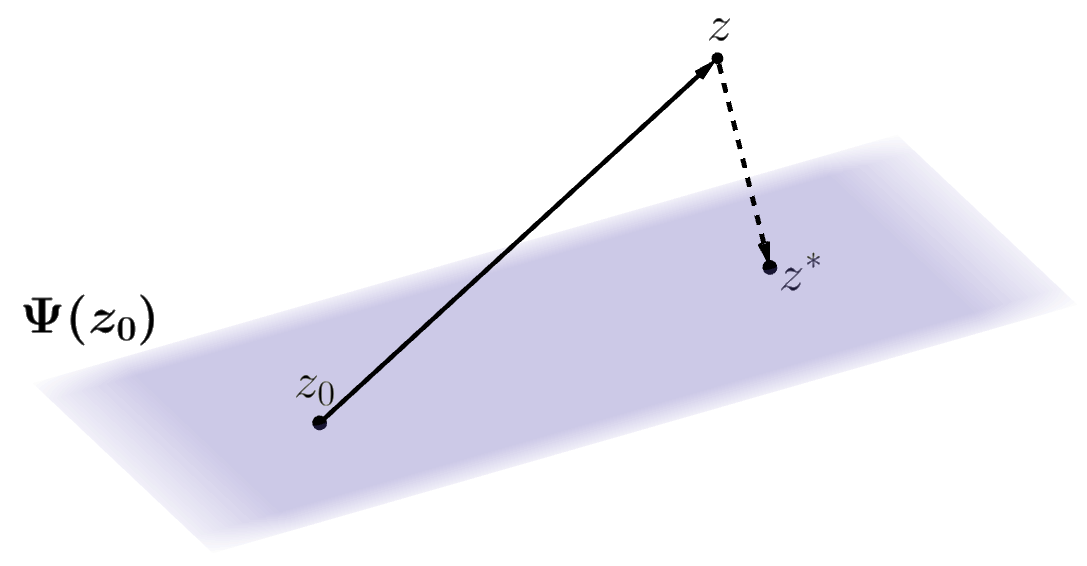
\includegraphics[width=0.5\linewidth]{tcc//img/corretor_visualizacao.png}
    \caption{Representação visual do corretor numérico.}
    \label{fig:corretor_visualizacao}
\end{figure}

Tome uma função $f(\vet x) = \frac{1}{2} \norma{\tilde{\vet z} - \vet x}^2$, cujo problema de otimização é equivalente a (\ref{eq:problema_otimizacao_corretor}). O processo se torna o método de quadrados mínimos. Tome $\vet y$ um candidato a mínimo do problema. As condições necessárias de otimização para o problema implicam que nesse caso \citep{Friedlander1994}:
\begin{equation}\label{eq:corretor_equacao_1}
    \nabla f(\vet y) = \tilde{\vet z} - \vet y
    = \sum_{i=1}^k \alpha_i \nabla \psi_i (\vet y) = D \vet \Psi (\vet y)^T \vet \alpha, 
    \quad \vet \alpha = (\alpha_1, ..., \alpha_k),
\end{equation}
onde $D \vet \Psi (\vet y)$ é a matriz jacobiana do campo vetorial de integrais primeiras e $\vet \alpha$ é o vetor de multiplicadores de Lagrange. Observe que a função objetivo $f$ é uma função convexa, e logo a condição necessária é também suficiente para o problema. Por Taylor, tem-se que
\begin{equation*}
    \vet \Psi (\tilde{\vet z}) \approx \vet \Psi (\vet y) + D \vet \Psi(\vet y) (\tilde{\vet z} - \vet y),
\end{equation*}
o que pela equação (\ref{eq:corretor_equacao_1}) pode ser escrito como:
\begin{equation}\label{eq:corretor_equacao_2}
    D \vet \Psi(\vet y) D \vet \Psi(\vet y)^T \vet \alpha 
    \approx
    \vet \Psi (\tilde{\vet z}) - \vet \Psi(\vet y)
    = 
    \vet \Psi (\tilde{\vet z}) - \vet \Psi(\vet z_0).
\end{equation}

Resolvendo (\ref{eq:corretor_equacao_2}) obtém-se os multiplicadores de Lagrange, que podem ser substituídos em (\ref{eq:corretor_equacao_1}):
\begin{equation*}
    \vet y = \tilde{\vet z} - D \vet \Psi(\vet y)^T \vet \alpha \approx \vet z^*.
\end{equation*}

Dessa forma, ainda que seja utilizado um método tradicional, é possível obter uma solução que preserve \textit{razoavelmente} as integrais primeiras. Essa \textit{razoabilidade} está ligada com o tamanho de passo $h$ escolhido da maneira como segue.

Considere um problema local no instante $t_n$ dado por
\begin{equation*}
    \dvet u (t) = F(t, \vet u(t)), \quad \vet u(t_n) = \vet z_n^*,
\end{equation*}
onde $\vet z_n$ é uma aproximação para o problema original no instante $t_n$ que satisfaz as integrais primeiras. Um tamanho de passo $h$ está relacionado a um erro local $\tau$ de modo que
\begin{equation*}
    \norma{u(t_{n+1}) - \vet z_{n+1}} \leq \tau.
\end{equation*}
Tomando uma aproximação corrigida $\vet z_{n+1}^*$, observe que
\begin{align*}
    \norma{\vet z(t_{n+1}) - \vet z_{n+1}^*} 
    & = \norma{\vet z(t_{n+1}) - \vet u(t_{n+1}) + \vet u(t_{n+1}) - \vet z_{n+1} + \vet z_{n+1} - \vet z_{n+1}^*} \\
    & \leq \norma{\vet z(t_{n+1}) - \vet u(t_{n+1})} + \norma{\vet u(t_{n+1}) - \vet z_{n+1}} + \norma{\vet z_{n+1} - \vet z_{n+1}^*} \\
    & \leq \zeta_h + \tau + \mu,
\end{align*}
onde $\zeta_h$ limita a norma de $\vet z(t_{n+1}) - \vet u(t_{n+1})$ e $\mu = \norma{\vet z_{n+1} - \vet z_{n+1}^*}$. A constante $\zeta_h$ é garantida por $f$ ser Lipschitz com constante $L$:
\begin{equation*}
    \norma{\vet z(t_{n+1}) - \vet u(t_{n+1})} \leq e^{h L} \norma{\vet z(t_n) - \vet z_n^*} = \zeta_h.
\end{equation*}
Quanto à $\mu$, se garantida sua existência como constante, então aplicar a correção sobre uma aproximação com erro $\tau$ possui um erro de discretização equivalente a não aplicar a correção sobre uma aproximação de erro $\tau + \mu$. 

Observe que $\vet u(t)$ satisfaz as integrais primeiras, pois seu valor inicial $\vet z_n^*$ as satisfaz. Em particular $\vet u(t_{n+1}) = \vet z_{n+1}^*$ satisfaz, e logo a correção é tal que $\mu = \tau$, o que significa que aplicá-la sobre uma aproximação de ordem $p$ fornece uma aproximação corrigida também de ordem $p$. Dessa forma, o corretor preserva a ordem do integrador.

Quanto à aplicação computacional, algumas questões merecem ser tratadas, e constam na seção \ref{secao:uso_do_corretor}.